\documentclass[article,a4paper,firamath,12pt]{nsi}
\usepackage{ulem}
\setminted{fontsize=\small}
\begin{document}
\titre{Préparation DS 02}
\classe{NSI2}
\maketitle
\setminted{fontsize=\small}
\subsection*{Exercice 1 : BDD}
Afin de lancer un nouveau service de streaming de musique, vous devez construire une base de données pour les morceaux de votre catalogue. Pour l'instant vous disposez d'une seule table avec les informations des morceaux. Voici \textbf{un extrait} de cette table :
\begin{center}\tabstyle[UGLiOrange]
    \scriptsize
    \begin{tabular}{|c|c|c|c|c|c|c|}
        \hline
        \rowcolor{UGLiOrange} \color{white}\textbf{Titre} & \color{white}\textbf{Durée} & \color{white}\textbf{Artiste}            & \color{white}\textbf{Album} & \color{white}\textbf{Piste} & \color{white}\textbf{CD} & \color{white}\textbf{Année} \\
        \hline
        Astronomy                                         & 384                         & Blue Öyster Cult                         & Secret Treaties             & 8                           & 1                        & 1974                        \\
        \hline
        Stone Cold Crazy                                  & 136                         & Queen                                    & Sheer Heart attack          & 8                           & 1                        & 1974                        \\
        \hline
        Under Pressure                                    & 242                         & Queen and David Bowie                    & Hot Space                   & 11                          & 2                        & 1982                        \\
        \hline
        The Outlaw Torn                                   & 589                         & Metallica                                & Load                        & 14                          & 1                        & 1996                        \\
        \hline
        Fuel                                              & 270                         & Metallica                                & Reload                      & 1                           & 1                        & 1997                        \\
        \hline
        The Memory Remains                                & 279                         & Metallica and Marianne Faithfull         & Reload                      & 2                           & 1                        & 1997                        \\
        \hline
        Astronomy                                         & 398                         & Metallica                                & Garage Inc.                 & 8                           & 1                        & 1998                        \\
        \hline
        Stone Cold Crazy                                  & 139                         & Metallica                                & Garage Inc.                 & 11                          & 2                        & 1998                        \\
        \hline
        Fuel                                              & 276                         & Metallica and the San Francisco Symphony & S\&M                        & 6                           & 1                        & 1999                        \\
        \hline
        The Outlaw Torn                                   & 599                         & Metallica and the San Francisco Symphony & S\&M                        & 6                           & 2                        & 1999                        \\
        \hline
    \end{tabular}
\end{center}
Cette table ne convient pas vraiment pour faire une base de données.

\textbf{1.} Expliquer pourquoi aucune des colonnes ne peut pas servir de clef primaire.\\

\carreauxseyes{16.8}{4}

\textbf{2.} Pourquoi est-ce que cette table est problématique si on veut rajouter des informations sur les artistes, comme leur nationalité ?\\

\carreauxseyes{16.8}{3.2}\\
\newpage
\textbf{3.} Quel est le problème si on souhaite chercher les morceaux d'un artiste ? Vous pourrez prendre l'exemple de Metallica.\\	

\carreauxseyes{16.8}{4}\\

Un ami vous suggère d'utiliser le schéma suivant :\\

\textbf{Morceau}(\uline{titre\_id}, titre, duree, \dashuline{artiste\_id}, album, piste, cd, annee)\\
\textbf{Artiste}(\uline{artiste\_id}, nom)\\

\textbf{4.}	Expliquer pourquoi cette représentation ne permet toujours pas de gérer les morceaux fait par deux artistes différents.	\\

\carreauxseyes{16.8}{4}\\


Finalement, vous arrivez au schéma suivant :
\begin{center}
    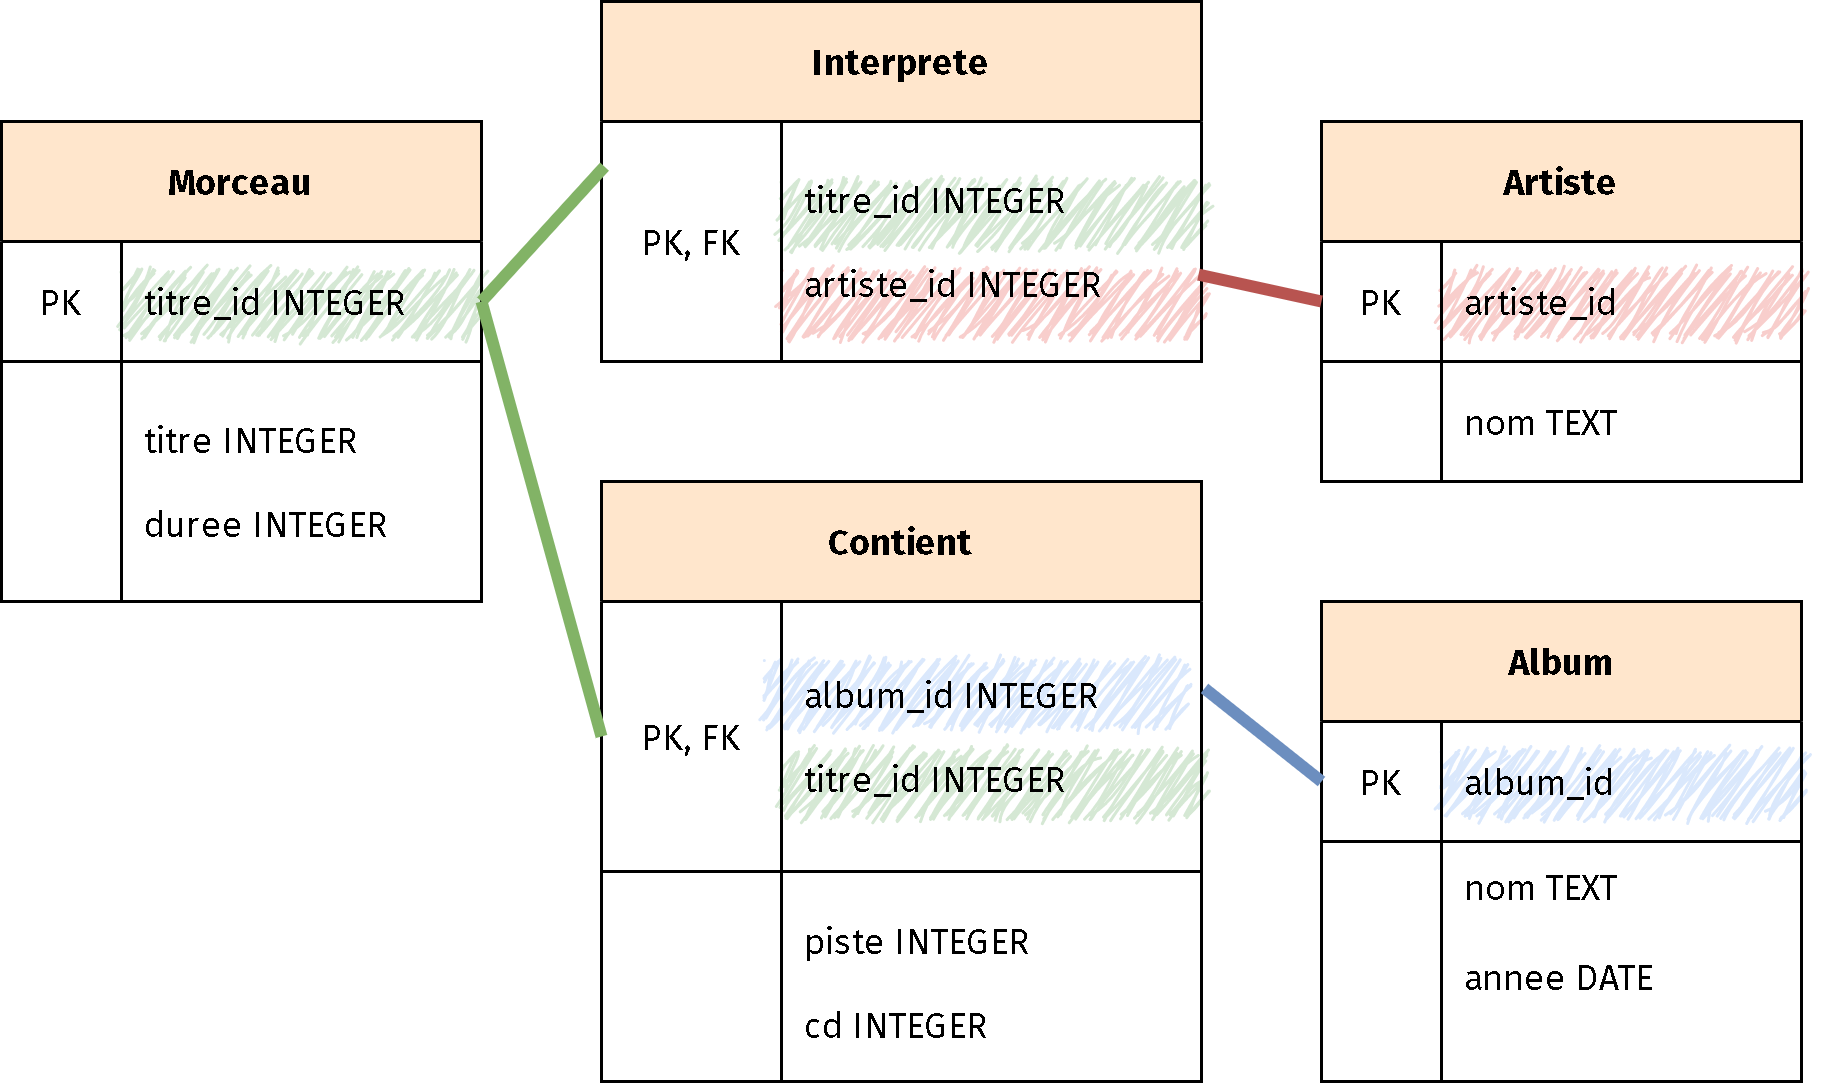
\includegraphics[width=12cm]{img/schema}
\end{center}

\textbf{5.}	Compléter les tables à l'aide des informations déjà disponibles. Un des morceaux n'a pas été intégré, inutile de l'y remettre. Si les noms dépassent, mettre uniquement le début.

\begin{center}
    \small
    \tabstyle[UGLiOrange]
    \begin{tabular}{|c|c|c|}
        \hline
        \rowcolor{UGLiOrange} \color{white}\textbf{titre\_id} & \color{white}\textbf{titre} & \color{white}\textbf{duree} \\
        \hline
        519                                                   & Astronomy                   & \color{white}384            \\
        \hline
        1219                                                  & Astronomy                   & \color{white}398            \\
        \hline
        316                                                   & Stone Cold Crazy            & 136                         \\
        \hline
        1319                                                  & Stone Cold Crazy            & 139                         \\
        \hline
        1298                                                  & \color{white}Fuel           & 270                         \\
        \hline
        1570                                                  & \color{white}Fuel           &                             \\
        \hline
        401                                                   & \color{white}Under Pressure &                             \\
        \hline
        1125                                                  & The Outlaw Torn             & 589                         \\
        \hline
        599                                                   & The Outlaw Torn             & 599                         \\
        \hline
    \end{tabular}\hspace*{1em}
    \begin{tabular}{|c|c|}
        \hline
        \rowcolor{UGLiOrange} \color{white}\textbf{titre\_id} & \color{white}\textbf{artiste\_id} \\
        \hline
        519                                                   & 25                                \\
        \hline
        1219                                                  & 154                               \\
        \hline
        1319                                                  & \color{white}154                  \\
        \hline
        1298                                                  & 154                               \\
        \hline
        1570                                                  & 154                               \\
        \hline
        1570                                                  & 318                               \\
        \hline
        1125                                                  & 154                               \\
        \hline
        1591                                                  & 154                               \\
        \hline
        1591                                                  & 318                               \\
        \hline
        316                                                   & 79                                \\
        \hline
        401                                                   & 79                                \\
        \hline
        401                                                   & 108                               \\
        \hline
    \end{tabular}	\hspace*{1em}
    \begin{tabular}{|c|c|}
        \hline
        \rowcolor{UGLiOrange} \color{white}\textbf{artiste\_id} & \color{white}\textbf{nom}     \\
        \hline
        \color{white} 154                                       & Metallica                     \\
        \hline
        318                                                     & \color{white}San Francisco S. \\
        \hline
        25                                                      & \color{white}Blue Öyster Cult \\
        \hline
        79                                                      & \color{white} Queen           \\
        \hline
        108                                                     & \color{white} David Bowie     \\
        \hline
    \end{tabular}
\end{center}
\textbf{6.} Comment appelle-t-on les clefs primaires de certaines tables apparaissant dans certaines tables, comme dans Interprete?\\

\carreauxseyes{16.8}{1.6}\\

\textbf{7.} Expliquer pourquoi le couple (titre\_id, artiste\_id) peut servir de clef primaire à Interprete.\\

\carreauxseyes{16.8}{3.2}\\

\textbf{8.} Traduire en langage naturel les requêtes suivantes :	

\begin{sql}
    \begin{minted}{sql}
    SELECT titre, duree FROM Morceau 
    WHERE duree > 600 
    ORDER BY duree DESC;
    \end{minted}
\end{sql}

\carreauxseyes{16.8}{2.4}\\

\begin{sql}
    \begin{minted}{sql}
        SELECT cd, piste, titre FROM Morceau
        JOIN Contient ON Contient.titre_id = Morceau.titre_id
        JOIN Album ON Contient.album_id = Album.album_id 
        WHERE nom = "Garage Inc."
        ORDER BY cd, piste;                
    \end{minted}
\end{sql}

\carreauxseyes{16.8}{2.4}\\

\textbf{9.} Donner la requête SQL permettant d'obtenir le nom de l'artiste dont l'identifiant est 200.\\

\carreauxseyes{16.8}{4}\\


\textbf{10.}	Donner la requête SQL permettant d'obtenir le nom de tous les albums sortis entre 1999 et 2010.\\

\carreauxseyes{16.8}{4}\\
\newpage
\textbf{11.}	Donner la requête SQL permettant d'obtenir le titre et la durée de tous les morceaux, triés par ordre décroissant de durée, de tous les morceaux de l'artiste dont l'identifiant est 200.\\

\carreauxseyes{16.8}{6.4}\\

\textbf{12.}	Les stars étant capricieuses, certaines veulent changer de nom. Donner la requête permettant à 'Maître Gims' de devenir 'Gims' dans la table des artistes.\\

\carreauxseyes{16.8}{4}\\


On rajoute maintenant les tables pour les utilisateurs :\\

\textbf{Utilisateur}(util\_id INTEGER , nom TEXT, e-mail TEXT, adresse TEXT)\\
\textbf{Ecoute}(id\_ecoute INTEGER, titre\_id TEXT, util\_id INTEGER, date DATE)\\

\textbf{13.}	Expliquer pourquoi le couple (titre\_id ,util\_id) ne peut pas être une clef primaire.\\

\carreauxseyes{16.8}{2.4}\\
\newpage
\textbf{14.}	Donner la requête SQL permettant d'ajouter l'utilisateur numéro 2179, qui s'appelle Bob
VHS, dont l'email est bob.vhs@hotmail.com et qui habite à New York.\\

\carreauxseyes{16.8}{2.4}\\

\textbf{15.}	Traduire le requête suivante en langage naturel :
\begin{sql}
    \begin{minted}{sql}
SELECT COUNT(DISTINCT titre) FROM Morceau
JOIN Ecoute ON Morceau.titre_id = Ecoute.titre_id 
WHERE date = "2020-12-12";
        \end{minted}
\end{sql}


\carreauxseyes{16.8}{2.4}\\

\subsection*{Exercice 2 : renverser une file avec une pile}

\'Ecrire en \textsc{Python} une fonction \pythoninline{renverse_file} qui
\begin{itemize}
    \item 	en entrée prend une file;
    \item 	ne renvoie rien mais \textbf{utilise une pile} pour renverser la file.
\end{itemize}
\begin{exemple}[ d'utilisation]
    \begin{minted}{python}
>>> print(F)
2 -> 3 -> 5 -> 1
>>> renverse_file(F)
>>> print(F)
1 -> 5 -> 3 -> 2
\end{minted}
\end{exemple}

\carreauxseyes{16.8}{8}

\subsection*{Exercice 3 : fonction mystere}
Pour désigner une pile on donnera ses éléments en partant du sommet vers le fond. Ainsi \pythoninline{2 : 1 : 3} représentera la pile 
\begin{center}
    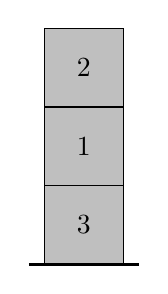
\begin{tikzpicture}
        \draw[fill=lightgray] (0,0) rectangle (1,1) rectangle (0,2)rectangle (1,3);
        \draw[thick] (-.2,0)--(1.2,0);
        \node (A) at (.5,.5) {3};
        \node (B) at (.5,1.5) {1};
        \node (C) at (.5,2.5) {2};
    \end{tikzpicture}
\end{center}

On considère la fonction suivante:

\begin{pyc}
    \begin{minted}{python}
def mystere(pile1, pile2):
    if est_vide(pile1):
        return pile2
    else:
        empiler(pile2, depiler(pile1))       
        return mystere(pile1, pile2)       
    \end{minted}
\end{pyc}


\textbf{1.} Dans cette question on a \pythoninline{p = 30 : 20 : 10} et \pythoninline{q = 40 : 50 : 60}. Que renvoie l' appel \pythoninline{mystere(p,q)} ?\\

\carreauxseyes{16.8}{1.6}\\

\textbf{2.} Expliquer en une phrase la fonction \pythoninline{mystere}.\\

\carreauxseyes{16.8}{1.6}\\

\textbf{3.} Dans cette question on a \pythoninline{p = 10 : 20}.\\
Que se passe t-il lors de l'appel mystere(p , p) ?\\

\carreauxseyes{16.8}{4}\\

\subsection*{Exercice 4 : maximum d'une file}
\'Ecrire en \textsc{Python} une fonction \pythoninline{max_file} qui
\begin{itemize}
    \item 	en entrée prend une file \textbf{non vide} composée d'\pythoninline{int} \textbf{positifs};
    \item 	renvoie le maximum de cette file. Attention la file doit être remise dans l'état initial et \textbf{aucune autre structure de données} (pile, file, liste) ne doit être utilisée.
\end{itemize}

\begin{exemple}[ d'utilisation]
    \begin{minted}{python}
>>> print(F)
>>> 2 -> 3 -> 5 -> 1
>>> max_file(F)
>>> 5
>>> print(F)
>>> 2 -> 3 -> 5 -> 1
\end{minted}
\end{exemple}

\carreauxseyes{16.8}{12}

\subsection*{Exercice 4 : analyse de code et POO}

Tu viens d'être nommé développeur dans une entreprise qui gère les systèmes d'alarmes pour les maisons des particuliers.
Ton prédécesseur a commencé à écrire une classe \pythoninline{Alarme}, qui doit normalement répondre aux exigences suivantes :

\begin{itemize}
    \item   l'alarme peut être activée et désactivée;
    \item   chaque intrusion détectée doit être systématiquement consignée dans un journal;
    \item   en cas d'intrusion, si l'alarme est activée, un SMS doit être envoyé au centre de télésurveillance.
\end{itemize}

Son code et la documentation sont donnés en annexe.


\textbf{1.} On exécute le script suivant :

\begin{pyc}
    \begin{minted}{python}
    from alarme import Alarme
    
    alarme1 = Alarme("Loritz", "971971971", False)
    alarme2 = Alarme("Poincaré", "971971971", True)
    alarme1.intrusion()
    alarme1.activer()
    alarme1.intrusion()
    alarme1.desactiver()
    alarme2.intrusion()        
    \end{minted}
\end{pyc}

Donner les contenus des SMS envoyés.\\

\carreauxseyes{16.8}{4}

\textbf{2.} Que contient \pythoninline{alarme1.journal} à la fin du script ?\\

\carreauxseyes{16.8}{4}\\

\textbf{3.} En testant le code, on constate que lorsque l'alarme est désactivée les intrusions ne sont pas enregistrées dans le journal.\\
D'où vient l'erreur ? Proposer une correction.\\

\carreauxseyes{16.8}{6.4}\\

\textbf{4.} On constate que le journal de bord consigne parfois des envois de SMS que le centre n'a jamais reçus : le système a bien tenté de les envoyé mais l'envoi a échoué.\\
Proposer une correction du code telle que si l'envoi d'un SMS échoue, cela soit consigné dans le journal.\\

\carreauxseyes{16.8}{12}\\

\textbf{5.} \'Ecrire une méthode d'instance \pythoninline{efface_journal} qui efface le journal de l'instance.\\


\carreauxseyes{16.8}{4}
\end{document}
